% Version 2.7: June 2025 validated manuscript package.
\documentclass[final,5p,times]{elsarticle}

\usepackage[utf8]{inputenc}
\usepackage{amsmath,amssymb,amsfonts}
\usepackage{booktabs}
\usepackage{graphicx}
\usepackage{xcolor}
\usepackage{url}
\usepackage{array}
\usepackage{tabularx}
\usepackage[hidelinks]{hyperref}
\IfFileExists{stfloats.sty}{\usepackage{stfloats}}{}
\renewcommand{\ttdefault}{cmtt}
\setlength{\emergencystretch}{3em}

\journal{Sustainable Energy, Grids and Networks}
\graphicspath{{paper2.7/}}
\biboptions{sort&compress}

\newcommand{\dt}{\Delta t}
\newcommand{\EV}{\mathrm{EV}}
\newcommand{\BESS}{\mathrm{BESS}}
\newcommand{\DA}{\mathrm{DA}}
\newcommand{\RT}{\mathrm{RT}}
\newcommand{\GI}{\mathrm{GI}}
\newcommand{\PV}{\mathrm{PV}}
\newcommand{\TOU}{\mathrm{TOU}}
\newcommand{\PD}{\mathrm{PD}}
\newcommand{\NCD}{\mathrm{NCD}}
\newcommand{\SOC}{\mathrm{SOC}}
\newcommand{\RU}{\mathrm{RU}}
\newcommand{\RD}{\mathrm{RD}}
\newcommand{\SP}{\mathrm{SP}}
\newcommand{\NSP}{\mathrm{NSP}}
\newcommand{\WM}{\mathrm{WM}}
\newcommand{\NWM}{\mathrm{NWM}}
\newcommand{\net}{\mathrm{net}}
\newcommand{\ch}{\mathrm{ch}}
\newcommand{\dch}{\mathrm{dch}}
\newcommand{\actual}{\mathrm{actual}}
\newcommand{\hist}{\mathrm{hist}}
\newcommand{\req}{\mathrm{req}}
\newcommand{\load}{\mathrm{load}}
\newcommand{\calT}{\mathcal{T}}
\newcommand{\calH}{\mathcal{H}}
\newcommand{\calI}{\mathcal{I}}
\newcommand{\calK}{\mathcal{K}}
\newcommand{\pos}[1]{\left[#1\right]_{+}}
\providecommand{\sep}{; }

\begin{document}

\begin{frontmatter}

\title{Execution-Aware Multi-Market Value Stacking for Behind-the-Meter Campus EV Charging and Battery Storage}

\author[ucsd]{Yizhan Gu}
\ead{yizhangu@ucsd.edu}
\author[totalenergies]{Wente Zeng}
\ead{wente.zeng@totalenergies.com}
\author[totalenergies]{Hadi Eshraghi}
\ead{hadi.eshraghi@external.totalenergies.com}
\author[ucsd]{Jan Kleissl\corref{cor1}}
\ead{jkleissl@ucsd.edu}
\cortext[cor1]{Corresponding author.}

\affiliation[ucsd]{organization={Center for Energy Research, University of California San Diego},
  city={La Jolla}, postcode={92093}, state={CA}, country={USA}}
\affiliation[totalenergies]{organization={TotalEnergies},
  city={Houston}, state={TX}, country={USA}}

\begin{highlights}
\item Executed first-step accounting couples campus EV service, retail charges, and wholesale value.
\item Fixed DA commitments and signed RT adjustments form a consistent two-settlement model.
\item Rolling 24-h policies are validated against a full billing-period Perfect benchmark.
\item All 5,820 Rolling solves and all 19 physical, financial, and solver checks pass.
\item The oracle benchmark exceeds the best 24-h policy by 14.38\% in June 2025.
\end{highlights}

\begin{abstract}
Campus electric-vehicle (EV) charging and battery energy storage systems (BESS) can jointly supply behind-the-meter (BTM) flexibility, but gross wholesale revenue is not a sufficient performance metric because the same dispatch changes retail energy and demand charges. This paper develops an execution-aware mixed-integer model predictive control framework that co-optimizes unidirectional workplace EV charging and a bidirectional BESS across retail time-of-use energy, peak-demand, and non-coincident demand charges; EV user payments; day-ahead (DA) and real-time (RT) energy; and four ancillary-service products. The framework closes three gaps in existing value-stacking studies: it prevents double counting of EV and BESS flexibility through a shared physical deliverability envelope, preserves irreversible DA commitments through signed RT adjustments, and evaluates forecast and horizon value from executed first-step dispatch against a full billing-period oracle. A June 2025 UC San Diego case compares shrinking- and rolling-horizon 24-h policies under Perfect and Persistence EV information. The full-period oracle yields \$12,565.15 and exceeds the best 24-h policy by \$1,579.73 (14.38\%). Perfect information over a truncated horizon is not a full-period upper bound because BESS state, demand thresholds, and DA commitments are path dependent. All 5,820 Rolling DA/RT solves are accepted at a 1\% relative MIP gap, with no time-limit event and physical and settlement residuals below prescribed tolerances. The resulting contribution is a market-timeline-consistent and independently auditable methodology for quantifying the net, rather than gross, value of BTM EV--BESS participation.
\end{abstract}

\begin{keyword}
Electric vehicle charging \sep Battery energy storage \sep Model predictive control \sep Value stacking \sep Ancillary services \sep Demand charges \sep Behind-the-meter resources
\end{keyword}

\end{frontmatter}

\section{Introduction}
\label{sec:introduction}

FERC Order No.~2222 seeks to reduce barriers to distributed-energy-resource (DER) participation in organized wholesale markets and explicitly includes storage, solar, controllable demand, EVs, and charging equipment among candidate resources \cite{ferc2222}. For a campus or commercial site, however, market access does not by itself establish profitability. A resource can earn wholesale energy or ancillary-service (AS) revenue while simultaneously increasing retail time-of-use (TOU) cost or establishing a higher monthly demand peak.

Workplace EV charging adds a second complication. Without vehicle-to-grid operation, EVs are not physical storage. Their flexibility is the ability to shift nonnegative charging power while each vehicle is connected and still satisfy its departure-energy requirement. A BESS is bidirectional but limited by power, state of charge (SOC), efficiency, and throughput. When both assets share a meter, their local and market-facing actions must be co-optimized rather than valued independently.

This paper addresses that coordination problem for a measured UC San Diego workplace-charging portfolio. The same optimization contains EV service, BESS physics, a signed BTM meter, retail energy and demand charges, DA/RT energy settlement, and regulation-up, regulation-down, spinning-reserve, and non-spinning-reserve capacity. CAISO identifies these four AS products and requires certification and telemetry for participating generation and load \cite{caisoAncillary2026}. The model is an operational and accounting abstraction; it is not a substitute for a complete CAISO registration or performance-settlement study.

The central methodological choice is \emph{execution-aware accounting}. Each MPC call produces a future plan, but only the first 15-min decision is implemented. SOC, EV energy, demand thresholds, active DA commitments, and revenue accounts are then updated from that executed quantity. This avoids reporting profits from future plan entries that are overwritten by later MPC calls.

The scientific contributions are:
\begin{enumerate}
  \item \textbf{A non-double-counting multi-resource deliverability model.} Unidirectional EV load modulation and bidirectional BESS power share one signed retail meter, one energy position, and one AS capability envelope. Market capacity cannot be sold independently by each accounting channel.
  \item \textbf{A market-timeline-consistent execution layer.} Submitted DA energy and AS quantities become immutable RT parameters; signed RT variables represent increments or decrements, and the actual physical obligation is their sum. This replaces an artificial DA-tracking penalty with the economic logic of two settlement.
  \item \textbf{A billing-period validation benchmark for economic MPC.} Executed 15-min dispatch is compared with a full-period Perfect oracle under common physical and boundary conditions. This exposes horizon value separately from forecast value and provides a formal explanation for non-monotone Perfect/Persistence rankings in truncated MPC.
  \item \textbf{A complete net-value audit.} Wholesale energy and capacity revenue is reconciled with signed TOU settlement, incremental monthly demand charges, EV user payments, EV service, device states, and interval-level feasibility.
\end{enumerate}

The current paper reports the formally validated June 2025 EV--BESS base case. Measured building-load and PV series are retained for a parallel passive-DER sensitivity case, described mathematically in Section~\ref{sec:passive_der}, but their numerical results are not mixed with the validated base-case claims.

\section{Related work and research gap}
\label{sec:literature}

\subsection{EV charging flexibility and aggregators}
Classical smart-charging studies establish that EV load can be shifted to reduce system cost or grid impacts while respecting availability and energy requirements \cite{clement2010impact,sortomme2011optimal,gan2013optimal,richardson2013electric}. Aggregation models translate heterogeneous session constraints into a tractable fleet capability \cite{nazari2022updated,alTaha2025aggregateFlex}. AS studies often assume V2G or bidirectional vehicle power \cite{sortomme2012v2gAncillary,clairand2020ancillary}; the present work instead treats EVs as strictly unidirectional loads.

Two recent UCSD studies are the closest EV-method predecessors. Chen et al.~\cite{chen2024costoptimal} optimized workplace EV flexibility for demand-response participation with TOU and demand charges. Chen et al.~\cite{chen2026realtime} added real-time feedback under EV forecast uncertainty. The current paper extends that line to co-located BESS operation, wholesale DA/RT energy, four AS products, and executed two-settlement accounting.

\subsection{MPC for charging stations and multi-service storage}
MPC has been demonstrated for charging stations and grid-connected microgrids \cite{hermans2024implementation,klemets2024charging}. PV--BESS charging-station studies have used explicit or robust-explicit MPC for uncertainty and carbon objectives \cite{cabrera2022realtime,cabrera2024robust}. These studies show that EV--PV--BESS coordination and MPC are established concepts; neither is claimed as the novelty here.

BTM storage value stacking combines local and grid services but creates competing uses of limited power and energy \cite{chen2021valueStacking,raoufat2018bess,idomar2026stacked}. Santosuosso et al.~\cite{santosuosso2024sempc} jointly considered renewable energy, storage, energy trading, AS, and stochastic economic MPC. Warmerdam et al.~\cite{warmerdam2026power} coordinated PV, EVs, heat pumps, and BESS for reserve provision. These works motivate a precise novelty boundary.

\subsection{Research gap and novelty}
Table~\ref{tab:literature_gap} positions the contribution against the closest
application classes. Prior work provides strong treatments of EV smart
charging, BTM storage, PV--EV--BESS coordination, or energy/AS trading, but the
intersection of retail demand-charge state, US-style DA/RT settlement,
non-double-counted EV--BESS deliverability, executed first-step accounting, and
a billing-period oracle remains unresolved. The paper addresses that
intersection. It does not claim a new generic MPC solver or a new forecast; the
methodological novelty is the coupling and validation structure needed to make
multi-market BTM value claims physically and financially defensible.

\begin{table*}[!t]
\centering
\caption{Positioning relative to closely related application studies. A check mark indicates that the element is central to the cited formulation or validation.}
\label{tab:literature_gap}
\scriptsize
\begin{tabularx}{\textwidth}{@{}p{0.25\textwidth}cccccX@{}}
\toprule
Study & Uni-dir. EV service & BTM demand charges & Energy + AS & DA/RT commitment logic & Full-period oracle & Primary distinction \\
\midrule
Chen et al.~\cite{chen2024costoptimal,chen2026realtime} & $\checkmark$ & $\checkmark$ & -- & -- & -- & Workplace EV demand response under forecast uncertainty.\\
Cabrera-Tobar et al.~\cite{cabrera2022realtime,cabrera2024robust} & $\checkmark$ & -- & -- & -- & -- & Experimental PV--EV--BESS robust/explicit MPC.\\
Santosuosso et al.~\cite{santosuosso2024sempc} & -- & -- & $\checkmark$ & $\checkmark$ & -- & Stochastic renewable--BESS energy and AS trading.\\
Id omar et al.~\cite{idomar2026stacked} & -- & $\checkmark$ & $\checkmark$ & -- & -- & Experimental BTM BESS local/grid service stacking.\\
Warmerdam et al.~\cite{warmerdam2026power} & $\checkmark$ & -- & $\checkmark$ & -- & -- & PV, flexible loads, and BESS for aFRR.\\
This work & $\checkmark$ & $\checkmark$ & $\checkmark$ & $\checkmark$ & $\checkmark$ & Executed US retail--DA/RT--AS value with a shared EV--BESS envelope.\\
\bottomrule
\end{tabularx}
\end{table*}

\section{System, data, and operating sequence}
\label{sec:system}

\subsection{BTM portfolio}
Figure~\ref{fig:architecture} shows the system boundary. EVs and the BESS are active decision resources in the validated base case. The site meter connects the physical dispatch to retail charges and wholesale deliverability. Building load and PV are passive exogenous additions in the planned sensitivity case.

\begin{figure*}[!t]
  \centering
  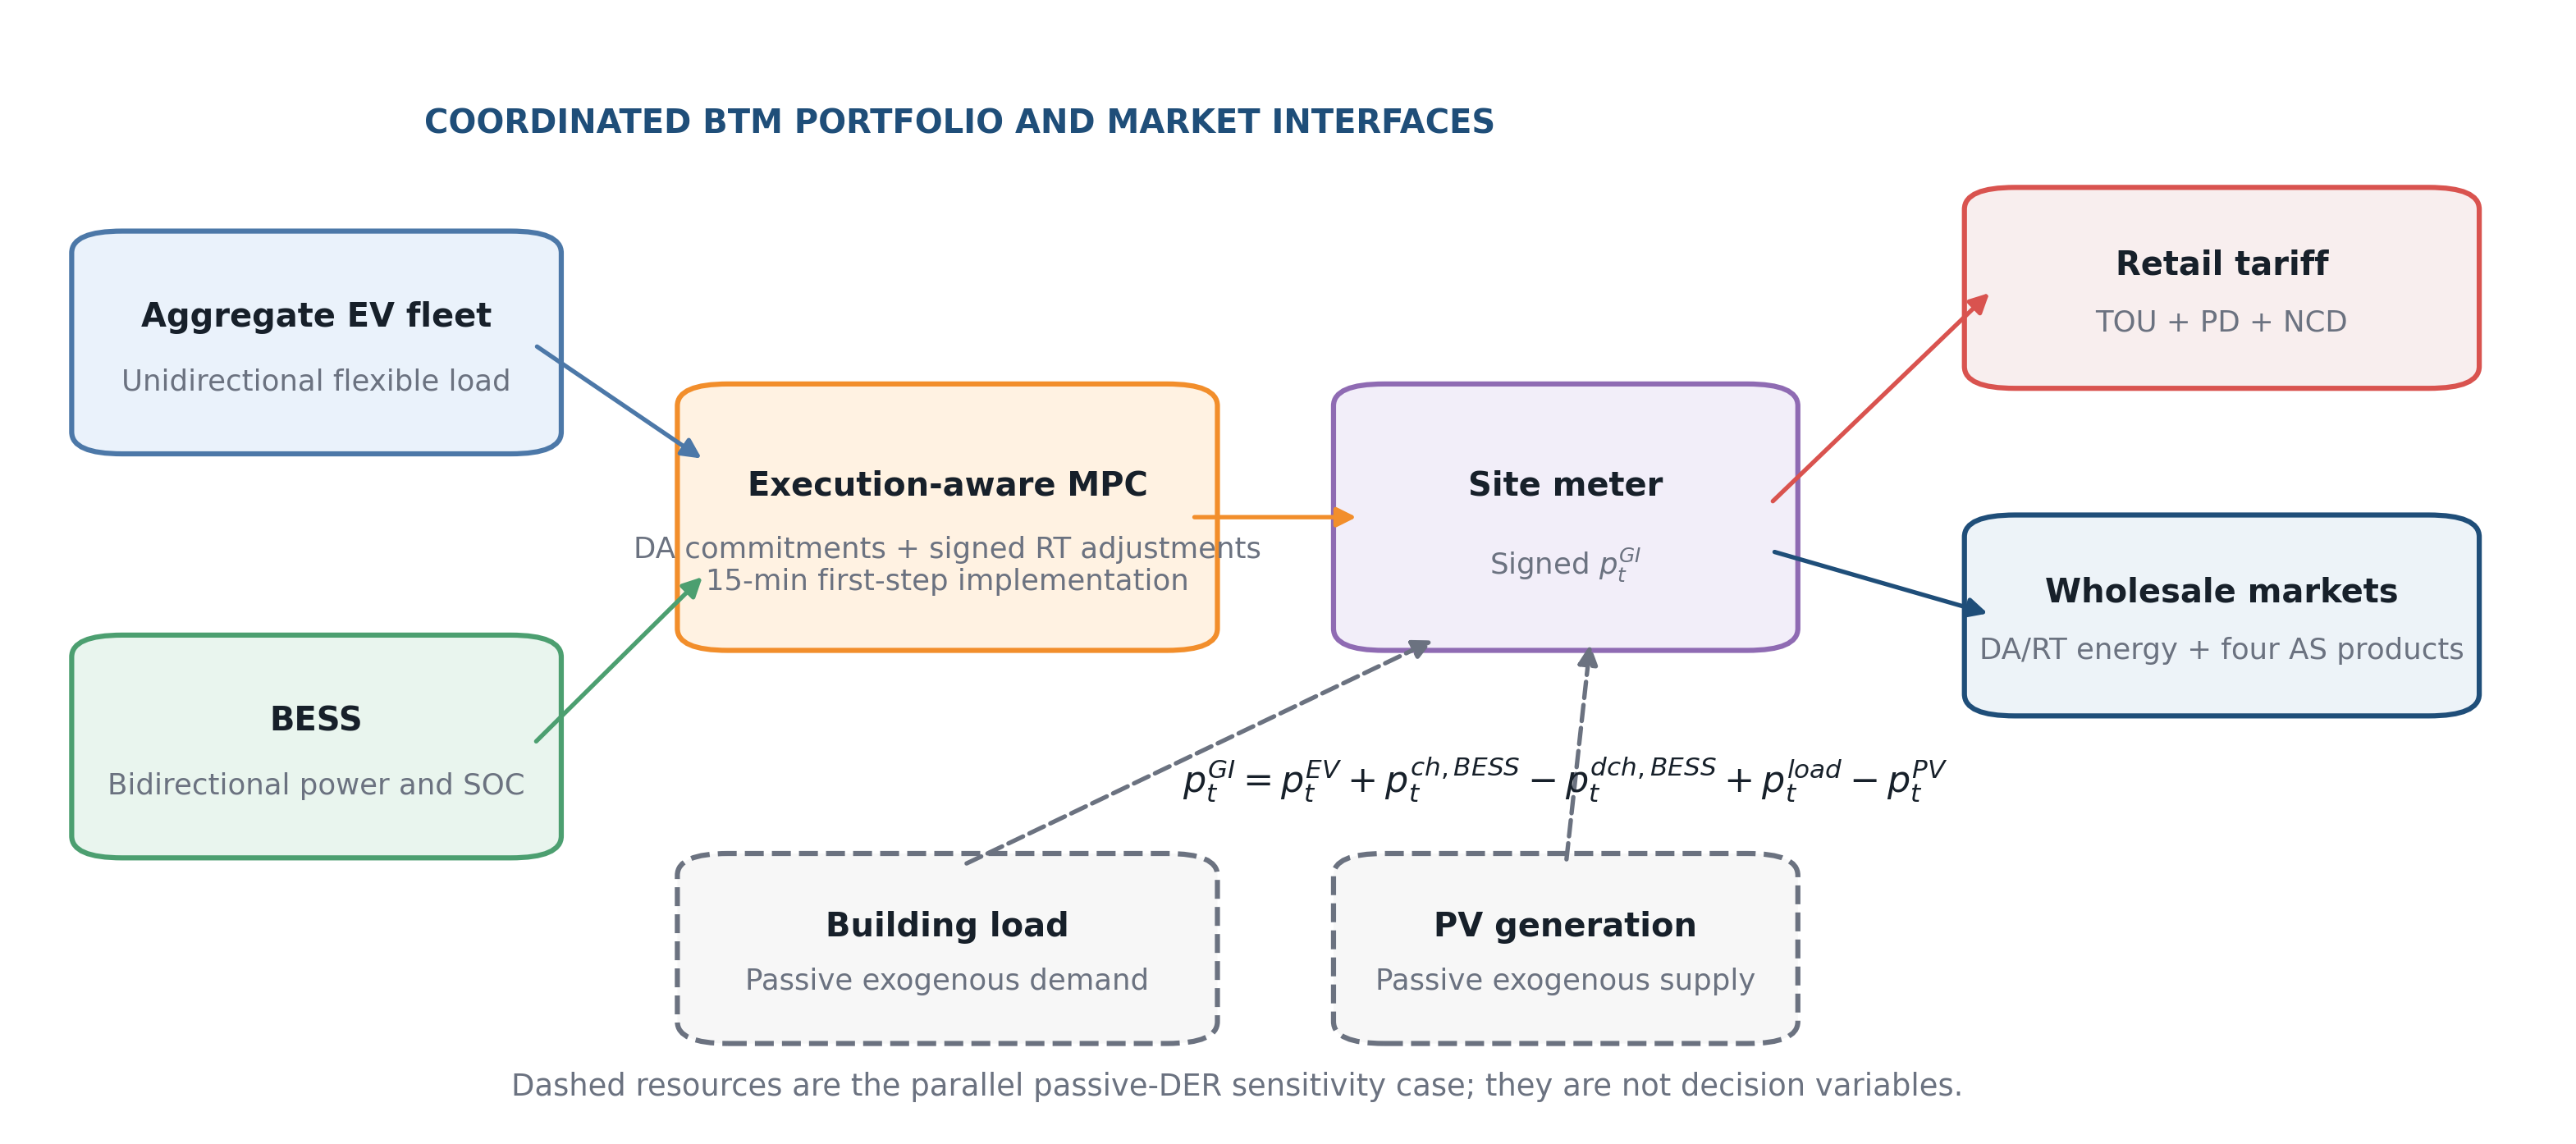
\includegraphics[width=0.96\textwidth]{fig_00_system_architecture.png}
  \caption{Campus BTM architecture. Solid boxes are active in the validated June EV--BESS base case. Dashed building-load and PV boxes define the parallel passive-DER sensitivity case and do not introduce new control variables.}
  \label{fig:architecture}
\end{figure*}

The EV input is an aggregate representation of all modeled UCSD charging sessions rather than a station-by-station electrical topology. Each session retains arrival, departure, energy, and charger-limit constraints. Market prices, tariff schedules, and EV information are aligned to a 15-min time index.

\subsection{DA/RT and MPC sequence}
Figure~\ref{fig:timeline} separates financial commitment from physical execution. DA quantities are solved before operation and become fixed parameters in RT. Every 15 min, RT optimization updates the EV forecast and physical states, solves the active horizon, and implements one step.

\begin{figure*}[!t]
  \centering
  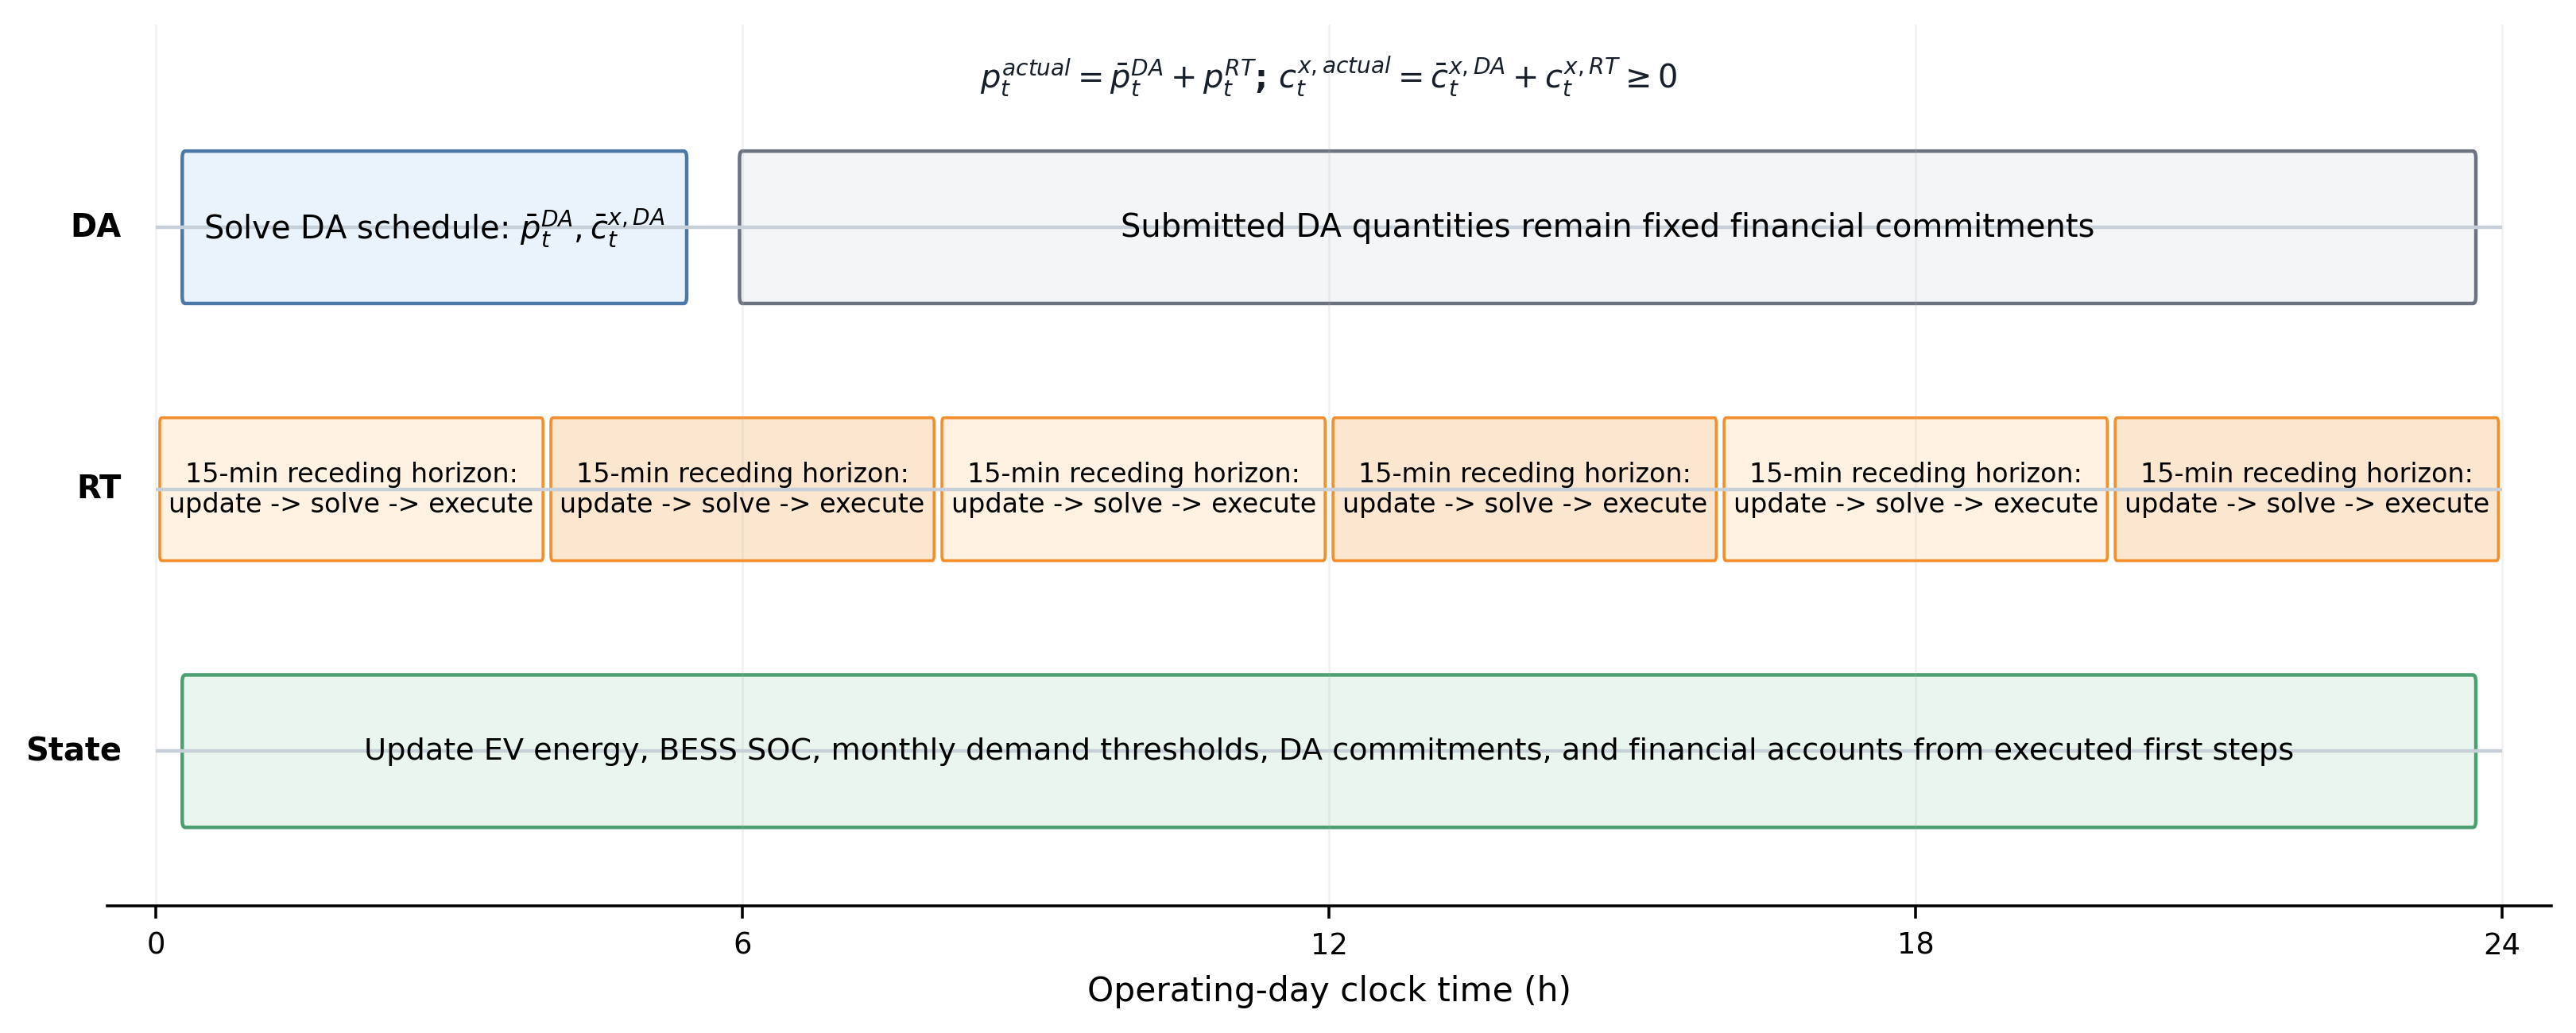
\includegraphics[width=0.96\textwidth]{fig_00_market_mpc_timeline.png}
  \caption{DA commitment, RT adjustment, and first-step MPC execution. Submitted DA quantities cannot be undone; RT variables change the actual position and are settled at RT prices.}
  \label{fig:timeline}
\end{figure*}

Two 24-h implementations are retained. Shrinking MPC optimizes the remaining service window, so its active horizon shortens as the day progresses. Rolling MPC advances a nominal 24-h window after each execution step. Both use the same device, meter, wholesale, and financial equations.

\section{Optimization model}
\label{sec:model}

\subsection{Sets, variables, and sign conventions}
Let $t\in\calT$ index 15-min intervals, $i\in\calI$ index EV sessions, and
$x\in\calK=\{\RU,\RD,\SP,\NSP\}$ index AS products. Positive
$p_t^{\GI}$ denotes site import and negative $p_t^{\GI}$ denotes export. Positive
market energy $p_t^{\actual}$ denotes upward delivery, while negative values
denote absorption. The positive-part operator is $\pos{z}=\max(z,0)$.

\begin{table*}[!t]
\centering
\caption{Core variables and parameters.}
\label{tab:notation}
\scriptsize
\begin{tabularx}{\textwidth}{@{}p{0.20\textwidth}X@{}}
\toprule
Symbol & Definition \\
\midrule
$p_{t,i}^{\EV}$, $p_t^{\EV}$ & EV-session charging power and fleet total; both are nonnegative.\\
$B_t^{\EV}$, $P_{t,\max}^{\EV}$ & EV baseline power and connected-fleet charging capability.\\
$p_t^{\ch,\BESS}$, $p_t^{\dch,\BESS}$, $s_t$ & BESS charge, discharge, and SOC.\\
$p_t^{\DA}$, $p_t^{\RT}$, $p_t^{\actual}$ & fixed DA energy, signed RT adjustment, and actual energy position.\\
$c_t^{x,\DA}$, $c_t^{x,\RT}$, $c_t^{x,\actual}$ & fixed DA AS, signed RT adjustment, and actual nonnegative AS capacity.\\
$M_k^{q,\hist}$ & executed billing-period threshold entering MPC call $k$, $q\in\{\PD,\NCD\}$.\\
$C_t^{\TOU}$, $C^q$ & retail energy and demand-charge rates.\\
$\lambda_t^{\DA}$, $\lambda_t^{\RT}$, $\rho_t^{x,s}$ & DA/RT energy and AS capacity prices.\\
\bottomrule
\end{tabularx}
\end{table*}

\subsection{EV service}
For availability $b_{t,i}\in\{0,1\}$, charger rating $\bar P_i$, charging
efficiency $\eta_i$, and required energy $E_i^{\req}$,
\begin{align}
0&\le p_{t,i}^{\EV}\le \bar P_i b_{t,i}, \label{eq:ev_power}\\
e_{t,i}&=e_{t-1,i}+\eta_i p_{t,i}^{\EV}\dt, \label{eq:ev_state}\\
e_{d_i,i}&=E_i^{\req},\qquad
p_t^{\EV}=\sum_i p_{t,i}^{\EV}. \label{eq:ev_service}
\end{align}
The equality in \eqref{eq:ev_service} prevents over- or under-service.
EV market flexibility is a deviation from $B_t^{\EV}$, not physical discharge:
\begin{align}
p_t^{\EV}-B_t^{\EV}
={}&(p_t^{\ch,\EV,\WM}-p_t^{\dch,\EV,\WM}) \nonumber\\
&+(p_t^{\ch,\EV,\NWM}-p_t^{\dch,\EV,\NWM}). \label{eq:ev_split}
\end{align}
Here $p_t^{\dch,\EV}$ means a reduction in EV load relative to baseline. It
never implies power export from a vehicle.

\subsection{BESS physics}
Let $C^{\BESS}$ be energy capacity, $P^{\BESS}$ power rating, and $\gamma$ the
round-trip efficiency parameter implemented through a square-root split:
\begin{align}
s_{t+1}
&=s_t+\frac{\dt}{C^{\BESS}}
\left(\sqrt{\gamma}\,p_t^{\ch,\BESS}
-\frac{p_t^{\dch,\BESS}}{\sqrt{\gamma}}\right), \label{eq:soc}\\
s^{\min}&\le s_t\le s^{\max}, \label{eq:soc_bounds}\\
0&\le p_t^{\ch,\BESS}\le P^{\BESS}u_t^{\ch}, \label{eq:bess_charge_power}\\
0&\le p_t^{\dch,\BESS}\le P^{\BESS}u_t^{\dch}, \label{eq:bess_discharge_power}\\
u_t^{\ch}+u_t^{\dch}&\le1. \label{eq:bess_direction}
\end{align}
A daily throughput guard is imposed separately for every calendar day
intersecting the active horizon. SOC carries between days; only the final
evaluation-period SOC is fixed:
\begin{align}
\dt\sum_{t\in\calT_d}
(p_t^{\ch,\BESS}+p_t^{\dch,\BESS})
&\le 2C^{\BESS}(s^{\max}-s^{\min}), \label{eq:throughput}\\
s_{T+1}&=s^{\mathrm{terminal}}. \label{eq:terminal}
\end{align}

\subsection{Meter balance and passive DER extension}
\label{sec:passive_der}
The general signed meter balance is
\begin{align}
p_t^{\GI}
=p_t^{\EV}+p_t^{\ch,\BESS}-p_t^{\dch,\BESS}
+p_t^{\load}-p_t^{\PV}. \label{eq:meter}
\end{align}
The validated base case sets $p_t^{\load}=p_t^{\PV}=0$. In the parallel
PV/building sensitivity, the two terms are measured or forecast exogenous
parameters. They are passive supply and demand, not new control variables. No
import/export split is added; the signed meter topology and all other
constraints remain unchanged.

\subsection{DA/RT energy and AS settlement}
Let $\bar p_t^{\DA}$ and $\bar c_t^{x,\DA}$ be submitted quantities and
$m_t$ an activation mask. In RT,
\begin{align}
p_t^{\DA}&=m_t\bar p_t^{\DA},&
p_t^{\actual}&=p_t^{\DA}+p_t^{\RT}, \label{eq:actual_energy}\\
c_t^{x,\DA}&=m_t\bar c_t^{x,\DA},&
c_t^{x,\actual}&=c_t^{x,\DA}+c_t^{x,\RT}\ge0. \label{eq:actual_as}
\end{align}
The RT variables are signed. Hence a negative $c_t^{x,\RT}$ can reduce an AS
award that cannot be fully delivered, but the actual provided quantity cannot
be negative.

With $P_{t,\max}^{\EV}=\sum_i\bar P_i b_{t,i}$, the common capability bounds are
\begin{align}
\bar P_t^{\mathrm{up}}&=P^{\BESS}+B_t^{\EV}, \label{eq:upbound}\\
\bar P_t^{\mathrm{down}}
&=\max\{P^{\BESS}-B_t^{\EV}+P_{t,\max}^{\EV},0\}. \label{eq:downbound}
\end{align}
The nonnegative clipping in \eqref{eq:downbound} is necessary when baseline EV
power exceeds the instantaneous BESS-plus-connected-EV absorption capability.
Actual energy and actual AS share these bounds:
\begin{align}
\pos{p_t^{\actual}}+
c_t^{\RU,\actual}+c_t^{\SP,\actual}+c_t^{\NSP,\actual}
&\le\bar P_t^{\mathrm{up}}, \label{eq:up_envelope}\\
\pos{-p_t^{\actual}}+c_t^{\RD,\actual}
&\le\bar P_t^{\mathrm{down}}. \label{eq:down_envelope}
\end{align}
The implementation also bounds $p_t^{\DA}$ and $p_t^{\RT}$ individually by the
same interval capability limits.

Expected AS deployment gives the market-facing power
\begin{align}
q_t^{\WM}={}&p_t^{\actual}
+\alpha_t^{\RU}c_t^{\RU,\actual}
-\alpha_t^{\RD}c_t^{\RD,\actual}\nonumber\\
&+\alpha_t^{\SP}c_t^{\SP,\actual}
+\alpha_t^{\NSP}c_t^{\NSP,\actual}. \label{eq:qwm}
\end{align}
Auxiliary net-flow variables satisfy
\begin{align}
p_t^{\dch,\net}&=\pos{q_t^{\WM}}, \label{eq:net_discharge}\\
p_t^{\ch,\net}&=\pos{-q_t^{\WM}}, \label{eq:net_charge}\\
p_t^{\ch,\net}-p_t^{\dch,\net}
={}&p_t^{\ch,\BESS,\WM}-p_t^{\dch,\BESS,\WM}\nonumber\\
&+p_t^{\ch,\EV,\WM}-p_t^{\dch,\EV,\WM}. \label{eq:net_link}
\end{align}
Direction binaries linearize \eqref{eq:net_discharge}--\eqref{eq:net_charge}. This is the role of
big-$M$ in the current model. The former big-$M$ penalty for following the DA
schedule is removed.

The conservative BESS duration guard for assumed duration $T^{\mathrm{DU}}$ is
\begin{align}
s_{t+1}&\ge s^{\min}
+\frac{T^{\mathrm{DU}}}{C^{\BESS}\sqrt{\gamma}}
\left(c_t^{\RU,\actual}+c_t^{\SP,\actual}\right.\nonumber\\
&\hspace{35mm}\left.+c_t^{\NSP,\actual}\right), \label{eq:duration_up}\\
s_{t+1}&\le s^{\max}
-\frac{T^{\mathrm{DU}}\sqrt{\gamma}}{C^{\BESS}}
c_t^{\RD,\actual}. \label{eq:duration_down}
\end{align}
The reference case uses $T^{\mathrm{DU}}=0.5$ h for all products as a modeling
assumption, not as a claim that every CAISO product has identical deployment
and certification rules.

\subsection{Retail costs}
The TOU term intentionally retains the signed meter:
\begin{align}
C_k^{\TOU}
=\sum_{t\in\calH_k}C_t^{\TOU}p_t^{\GI}\dt. \label{eq:tou}
\end{align}
Thus $p_t^{\GI}<0$ receives a retail-price export credit under the adopted
tariff convention.

For demand category $q\in\{\PD,\NCD\}$, let $M_k^{q,\hist}$ be the maximum
eligible executed import before solve $k$. The avoidable increase is modeled
with
\begin{align}
z_k^q&\ge0, \qquad
z_k^q\ge p_t^{\GI}-M_k^{q,\hist},
\quad t\in\calH_k\cap\calT_q, \label{eq:demand_epi}\\
C_k^{q,\mathrm{inc}}&=C^q z_k^q. \label{eq:demand_inc}
\end{align}
After executing interval $k$,
\begin{align}
M_{k+1}^{q,\hist}
=\max\{M_k^{q,\hist},\,m_q(k)p_k^{\GI,\mathrm{executed}}\}. \label{eq:threshold_update}
\end{align}
The earlier expression $C^q\max\{M_k^{q,\hist},\max_t p_t^{\GI}\}$ differs from
\eqref{eq:demand_inc} only by the constant $C^qM_k^{q,\hist}$ within a solve:
\begin{align}
C^q\max\{M,z\}=C^qM+C^q\pos{z-M}. \label{eq:demand_equivalence}
\end{align}
Therefore both yield the same optimizer when they use the same meter variable
and fixed historical threshold. Equation~\eqref{eq:demand_inc} is preferable
for incremental accounting because it does not repeatedly charge sunk cost.

\subsection{Wholesale revenue and objective}
Wholesale energy and AS capacity revenue are
\begin{align}
R_k^{\WM,\mathrm{energy}}
={}&\sum_{t\in\calH_k}\dt
\left(\lambda_t^{\DA}p_t^{\DA}
+\lambda_t^{\RT}p_t^{\RT}\right)+R_k^{\mathrm{deploy}}, \label{eq:wm_energy}\\
R_k^{\WM,\mathrm{capacity}}
={}&\sum_{t\in\calH_k}\dt\sum_{x\in\calK}
\left(\rho_t^{x,\DA}c_t^{x,\DA}
+\rho_t^{x,\RT}c_t^{x,\RT}\right), \label{eq:wm_capacity}\\
R_k^{\EV}
={}&\sum_{t\in\calH_k}C^{\EV}p_t^{\EV}\dt. \label{eq:ev_revenue}
\end{align}
$R_k^{\mathrm{deploy}}$ prices the expected deployment energy in
\eqref{eq:qwm} at the RT energy price.

At MPC call $k$, the complete active-horizon problem is
\begin{align}
\min_{\boldsymbol{x}_k\in\mathcal{X}(\mathcal{I}_k)}
J_k={}&
\sum_{t\in\calH_k}C_t^{\TOU}p_t^{\GI}\dt
+\sum_{q\in\{\PD,\NCD\}}C^qz_k^q \nonumber\\
&-R_k^{\EV}
-R_k^{\WM,\mathrm{energy}}
-R_k^{\WM,\mathrm{capacity}}, \label{eq:objective}
\end{align}
subject to \eqref{eq:ev_power}--\eqref{eq:duration_down} and the corresponding
binary linearizations. There is no DA-tracking penalty. The economic
consequence of deviating from DA is already represented by the DA/RT
two-settlement terms.

\section{Information policies, horizons, and oracle logic}
\label{sec:oracle_logic}

\subsection{Perfect and Persistence EV information}
Once a vehicle arrives, its realized session information is used. For sessions
that have not arrived, Perfect supplies the realized future session set within
the active horizon, while Persistence constructs the future set from recent
charging behavior. Electricity prices are exogenous processed inputs in both
cases; ``Perfect'' refers to EV information rather than to price forecasting.

\subsection{Why 24-h Perfect need not be best}
Let $\omega$ denote the complete realized billing-period data and
$\mathcal{X}(\omega)$ the common full-period feasible set. A true oracle solves
\begin{align}
J_{\mathrm{oracle}}^\star(\omega)
=\min_{\boldsymbol{x}\in\mathcal{X}(\omega)}
J_{\calT}(\boldsymbol{x};\omega). \label{eq:oracle}
\end{align}
For every feasible policy $\pi$,
\begin{align}
J_{\mathrm{oracle}}^\star\le J^\pi
\quad\Longleftrightarrow\quad
V_{\mathrm{oracle}}^\star\ge V^\pi,\qquad V=-J. \label{eq:oracle_dominance}
\end{align}
The inequality direction differs for cost and revenue.

A 24-h MPC policy instead solves
\begin{align}
\boldsymbol{x}_{k:k+H-1}^{\pi}\in
\arg\min_{\boldsymbol{x}}
\left[
\sum_{\tau=k}^{k+H-1}\ell_\tau
(\boldsymbol{x}_\tau;\mathcal{I}_k^\pi)
+\widehat V_{k+H}(s_{k+H})
\right], \label{eq:mpc}
\end{align}
executes only $\boldsymbol{x}_k^\pi$, and repeats. The current controller does
not know the exact continuation value $V_{k+H}^\star$. Consequently, more
accurate information inside the truncated horizon does not imply globally
better closed-loop value \cite{rawlings2017mpc}.

The mechanism resembles a greedy algorithm. Each solve selects a locally
attractive first action from incomplete future information. That action changes
the next state and therefore the feasible set of every later solve. Four state
channels matter here:
\begin{enumerate}
  \item BESS SOC and daily throughput usage;
  \item monthly PD and NCD thresholds;
  \item EV energy remaining before departure; and
  \item submitted DA energy and AS commitments that cannot be undone.
\end{enumerate}
A Persistence forecast can accidentally preserve a more valuable out-of-horizon
state than a Perfect 24-h solve. A 1\% MIP gap can also select different
near-optimal first actions and amplify their differences through the cascade,
but this is a secondary numerical mechanism. The validation rule is therefore:
the full-period oracle must dominate, while 24-h Perfect versus Persistence is
an empirical policy comparison.

\section{Case study and validation protocol}
\label{sec:case}

\subsection{June 2025 configuration}
The study covers 1--30 June 2025 at 15-min resolution. The BESS is rated at
250 kW and 332 kWh with SOC limits 0.05--0.95 and $\gamma=0.9$. The aggregate EV
charger limit is 6.6 kW per connected session. EV user revenue is \$0.40/kWh.
The summer PD and NCD rates are \$3.05/kW and \$15.38/kW, respectively. Gurobi
13.0.1 is called through CVXPY 1.8.2 with a 1\% relative MIP-gap target. The
formal Rolling run uses no ordinary per-step time limit; abnormal-run protection
is handled separately, and no TimeLimit event occurs.

All methods enter June from a common January--May baseline-state construction.
The full-period oracle uses the same Perfect baseline used by Rolling Perfect,
the same realized June input, the same physical constraints, and the same final
SOC target. Shrinking results provide the complete five-method financial
comparison, while detailed daily validation focuses on Rolling Persistence,
Rolling Perfect, and the full-period oracle because these three cases isolate
forecast and horizon effects under one controller structure.

\begin{table*}[!t]
\centering
\caption{Formal validation hierarchy and acceptance criteria.}
\label{tab:validation_protocol}
\scriptsize
\begin{tabularx}{\textwidth}{@{}p{0.27\textwidth}p{0.30\textwidth}X@{}}
\toprule
Layer & Criterion & Purpose \\
\midrule
Solver completeness & 30 DA + 2,880 RT solves per Rolling forecast; status optimal; gap $\le1\%$; no TimeLimit & Excludes silent truncation and missing intervals.\\
Physical identities & Meter, settlement, and actual up/down residuals $\le10^{-6}$ kW; actual AS $\ge-10^{-6}$ kW & Confirms the implemented dispatch matches the model.\\
EV service & Daily EV-energy spread across the three detailed scenarios $\le10^{-4}$ kWh & Prevents financial gains from unequal charging service.\\
Financial accounting & Daily component sum agrees with total within \$0.03 & Allows independent cent rounding but no missing account.\\
Terminal state & Final billing-period SOC equals 0.5 within $10^{-6}$ & Prevents end-of-study energy borrowing.\\
Oracle consistency & identical Rolling-Perfect baseline and oracle value not below Rolling Perfect & Establishes a comparable full-period benchmark.\\
Graphical audit & One rendered trajectory for every day & Links numerical checks to physical trajectories.\\
\bottomrule
\end{tabularx}
\end{table*}

\subsection{Computational validation}
The validation set contains 5,820 Rolling solves: two forecasts times 30 DA and
2,880 RT optimizations. Source identity, solver records, dispatch traces, daily
audits, and daily figures are archived together to prevent numerical results
from being separated from their implementation. All 19 acceptance checks pass.
The accepted full-period oracle terminates normally at a reported 0.8571\%
gap. A separate 900-s attempt found a higher feasible incumbent but stopped at
1.2006\%; it is retained as non-certified evidence and is not substituted into
the consistently certified result table.

\section{Results}
\label{sec:results}

\subsection{Monthly five-method comparison}
Table~\ref{tab:monthly_results} and Fig.~\ref{fig:monthly_stack} report executed
June results. Costs are stored as negative financial components, so
\begin{align}
V=R^{\EV}+R^{\WM}+C^{\TOU}+C^{\PD}+C^{\NCD}. \label{eq:financial_identity}
\end{align}

\begin{table*}[!t]
\centering
\caption{Executed June 2025 value decomposition (US\$).}
\label{tab:monthly_results}
\scriptsize
\begin{tabular}{@{}lrrrrrr@{}}
\toprule
Method & Net value & WM revenue & TOU & PD & NCD & EV revenue\\
\midrule
Full billing-period Perfect oracle & 12,565.15 & 4,564.69 & -10,404.95 & -114.85 & -4,873.66 & 23,393.92\\
Shrinking 24-h Persistence         & 10,985.42 & 4,424.62 & -11,527.35 & -527.59 & -4,778.15 & 23,393.92\\
Rolling 24-h Perfect              & 10,733.15 & 4,347.03 & -12,300.80 & -279.25 & -4,427.75 & 23,393.92\\
Shrinking 24-h Perfect            & 10,552.67 & 4,310.96 & -12,413.73 & -310.73 & -4,427.75 & 23,393.92\\
Rolling 24-h Persistence          & 10,485.28 & 4,421.87 & -11,092.27 & -467.84 & -5,770.41 & 23,393.92\\
\bottomrule
\end{tabular}
\end{table*}

\begin{figure*}[!t]
  \centering
  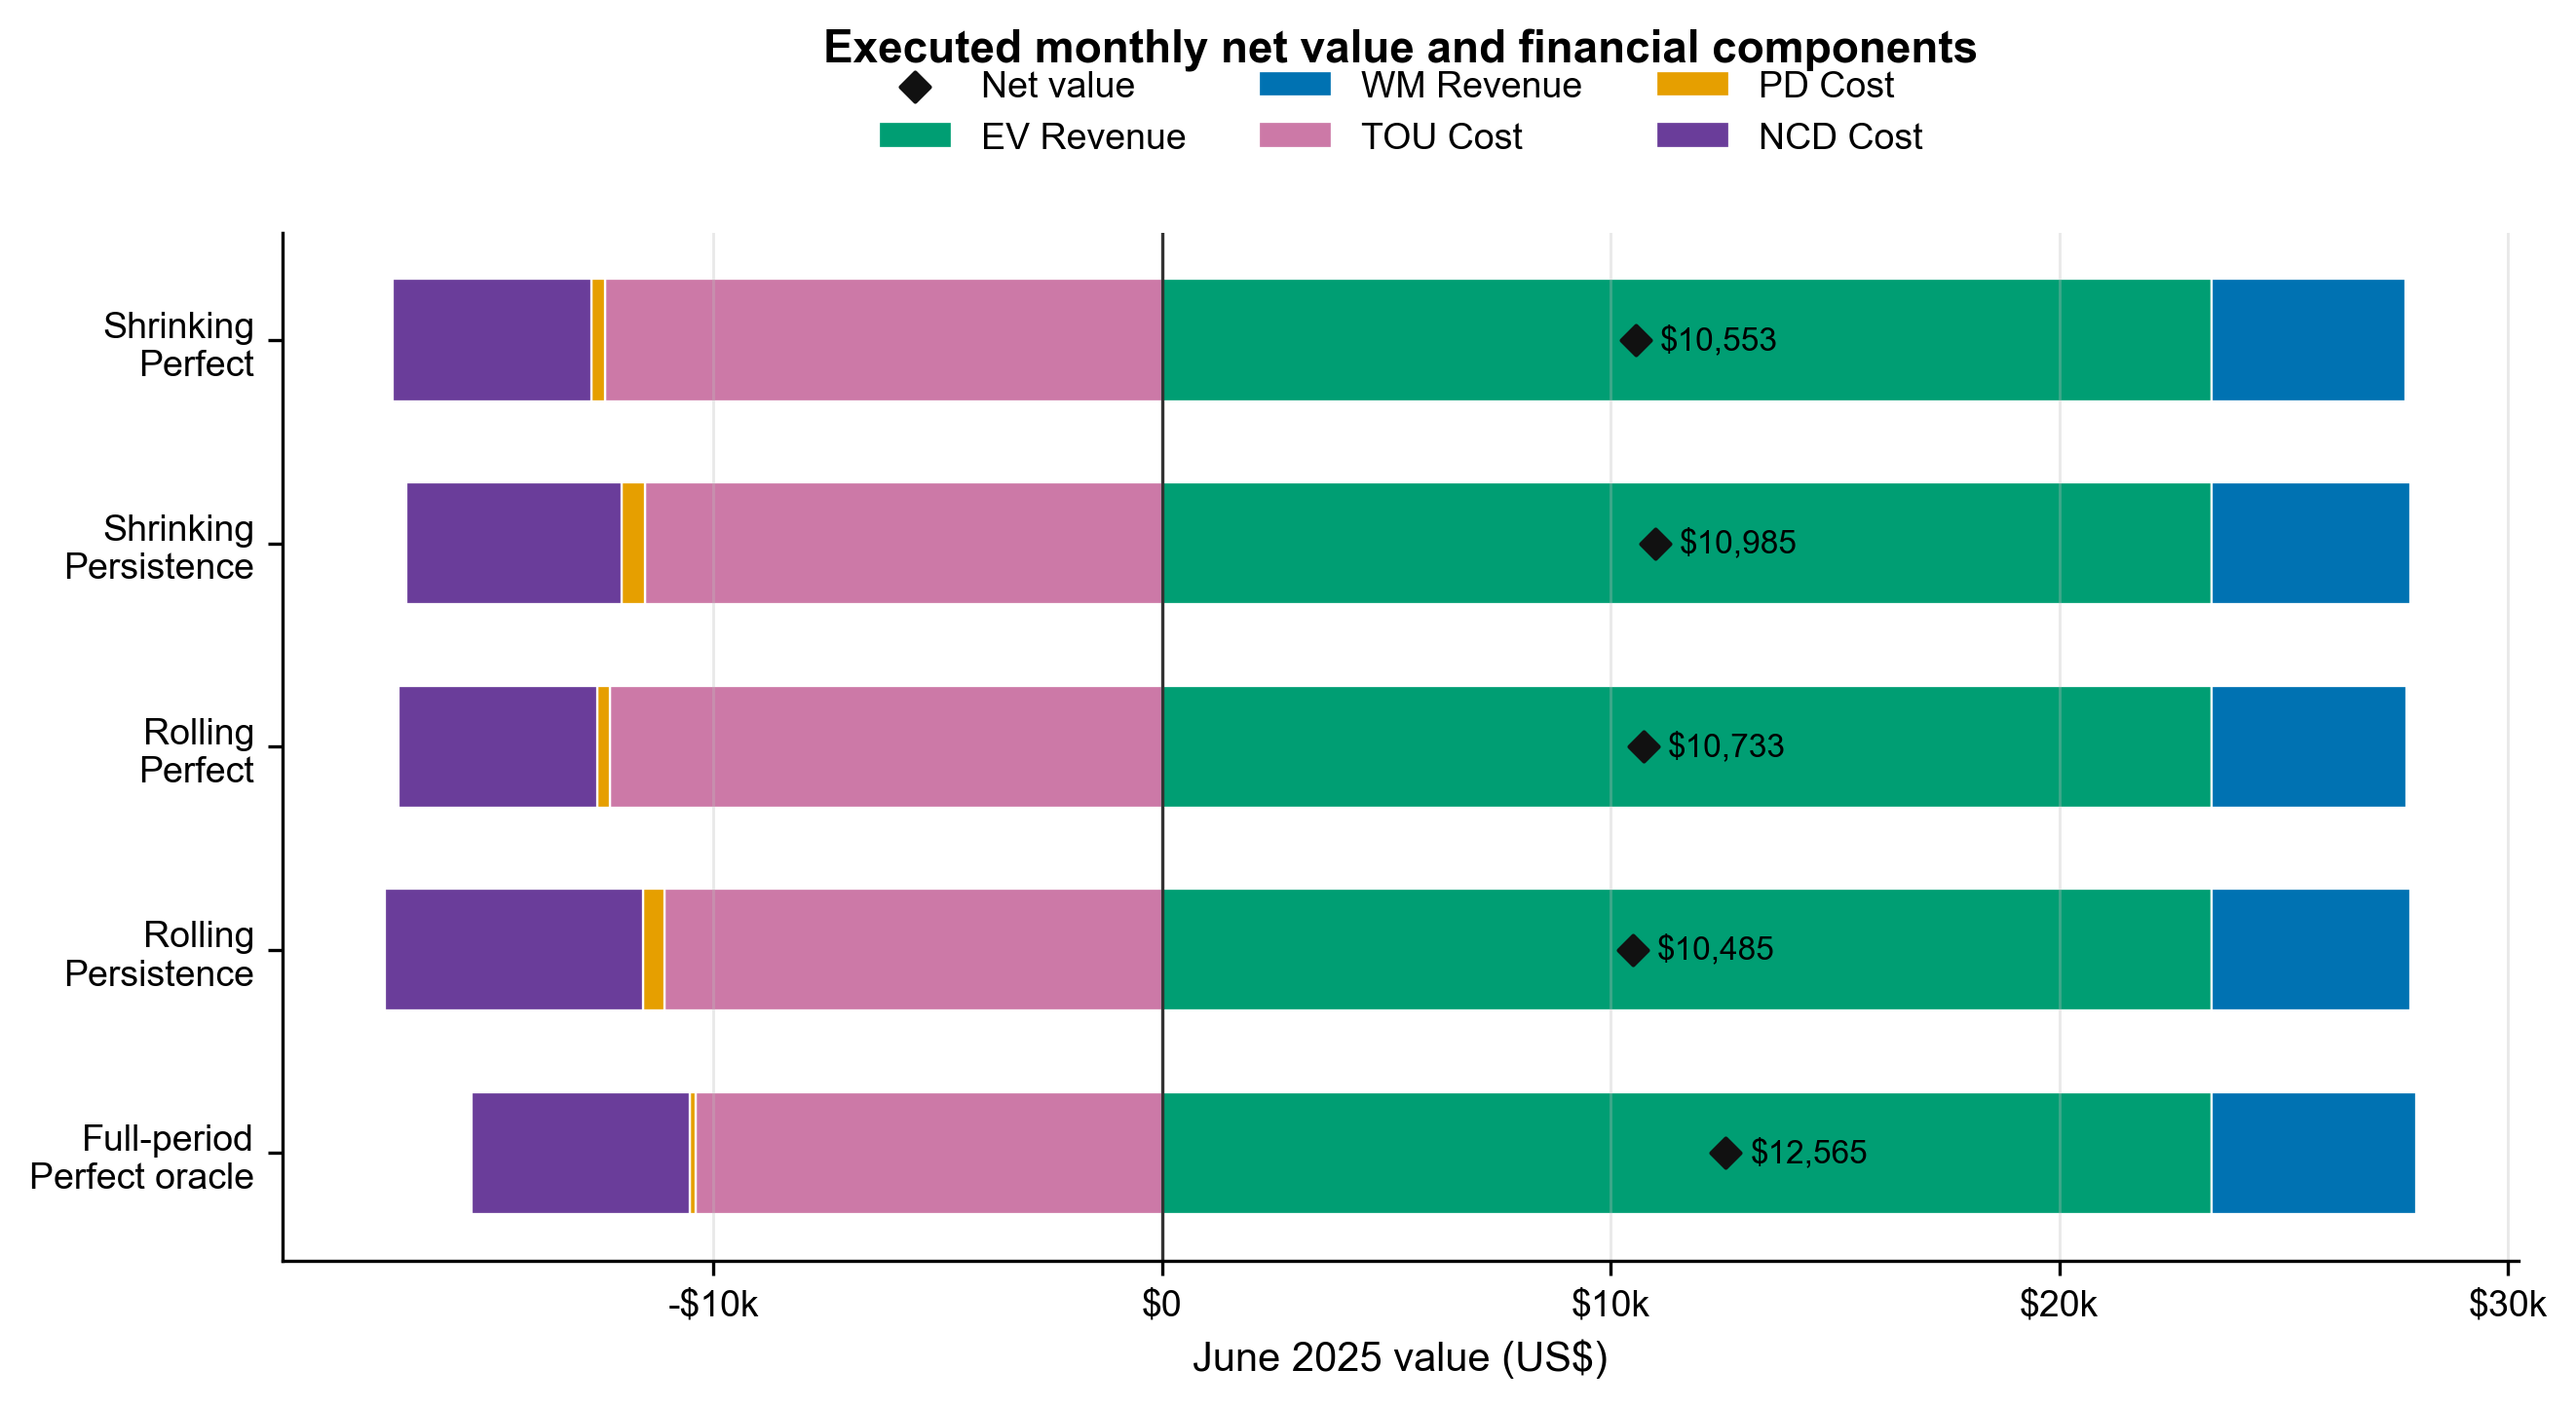
\includegraphics[width=0.96\textwidth]{fig_01_monthly_five_method_value_stack.png}
  \caption{June 2025 executed value stack. The identical EV-revenue component confirms equal aggregate service; method differences arise from wholesale and retail interactions.}
  \label{fig:monthly_stack}
\end{figure*}

The full-period oracle exceeds the best 24-h policy, Shrinking Persistence, by
\$1,579.73 or 14.38\%, and exceeds Rolling Perfect by \$1,832.00. The benefit is
not simply higher gross wholesale revenue. Relative to Rolling Perfect, the
oracle gains \$217.66 in WM revenue and reduces TOU cost by \$1,895.85, while
its NCD cost is \$445.91 larger. The net improvement is therefore a
retail--wholesale scheduling effect across the complete billing period.

The 24-h ordering is not monotonic in forecast quality. Perfect exceeds
Persistence by \$247.87 under Rolling MPC, whereas Persistence exceeds Perfect
by \$432.75 under Shrinking MPC. Section~\ref{sec:oracle_logic} shows why this is
permissible: forecast information, horizon, and path-dependent state jointly
determine the executed policy. These values are empirical results, not a
universal controller ranking.

\subsection{Daily financial mechanism}
Figure~\ref{fig:daily_financial} separates daily attributed and cumulative value
for the three detailed validation methods. Large negative daily values occur
when a new monthly demand maximum is established; they should not be interpreted
as an independent daily tariff. The cumulative plot is the appropriate
billing-period comparison.

\begin{figure*}[!t]
  \centering
  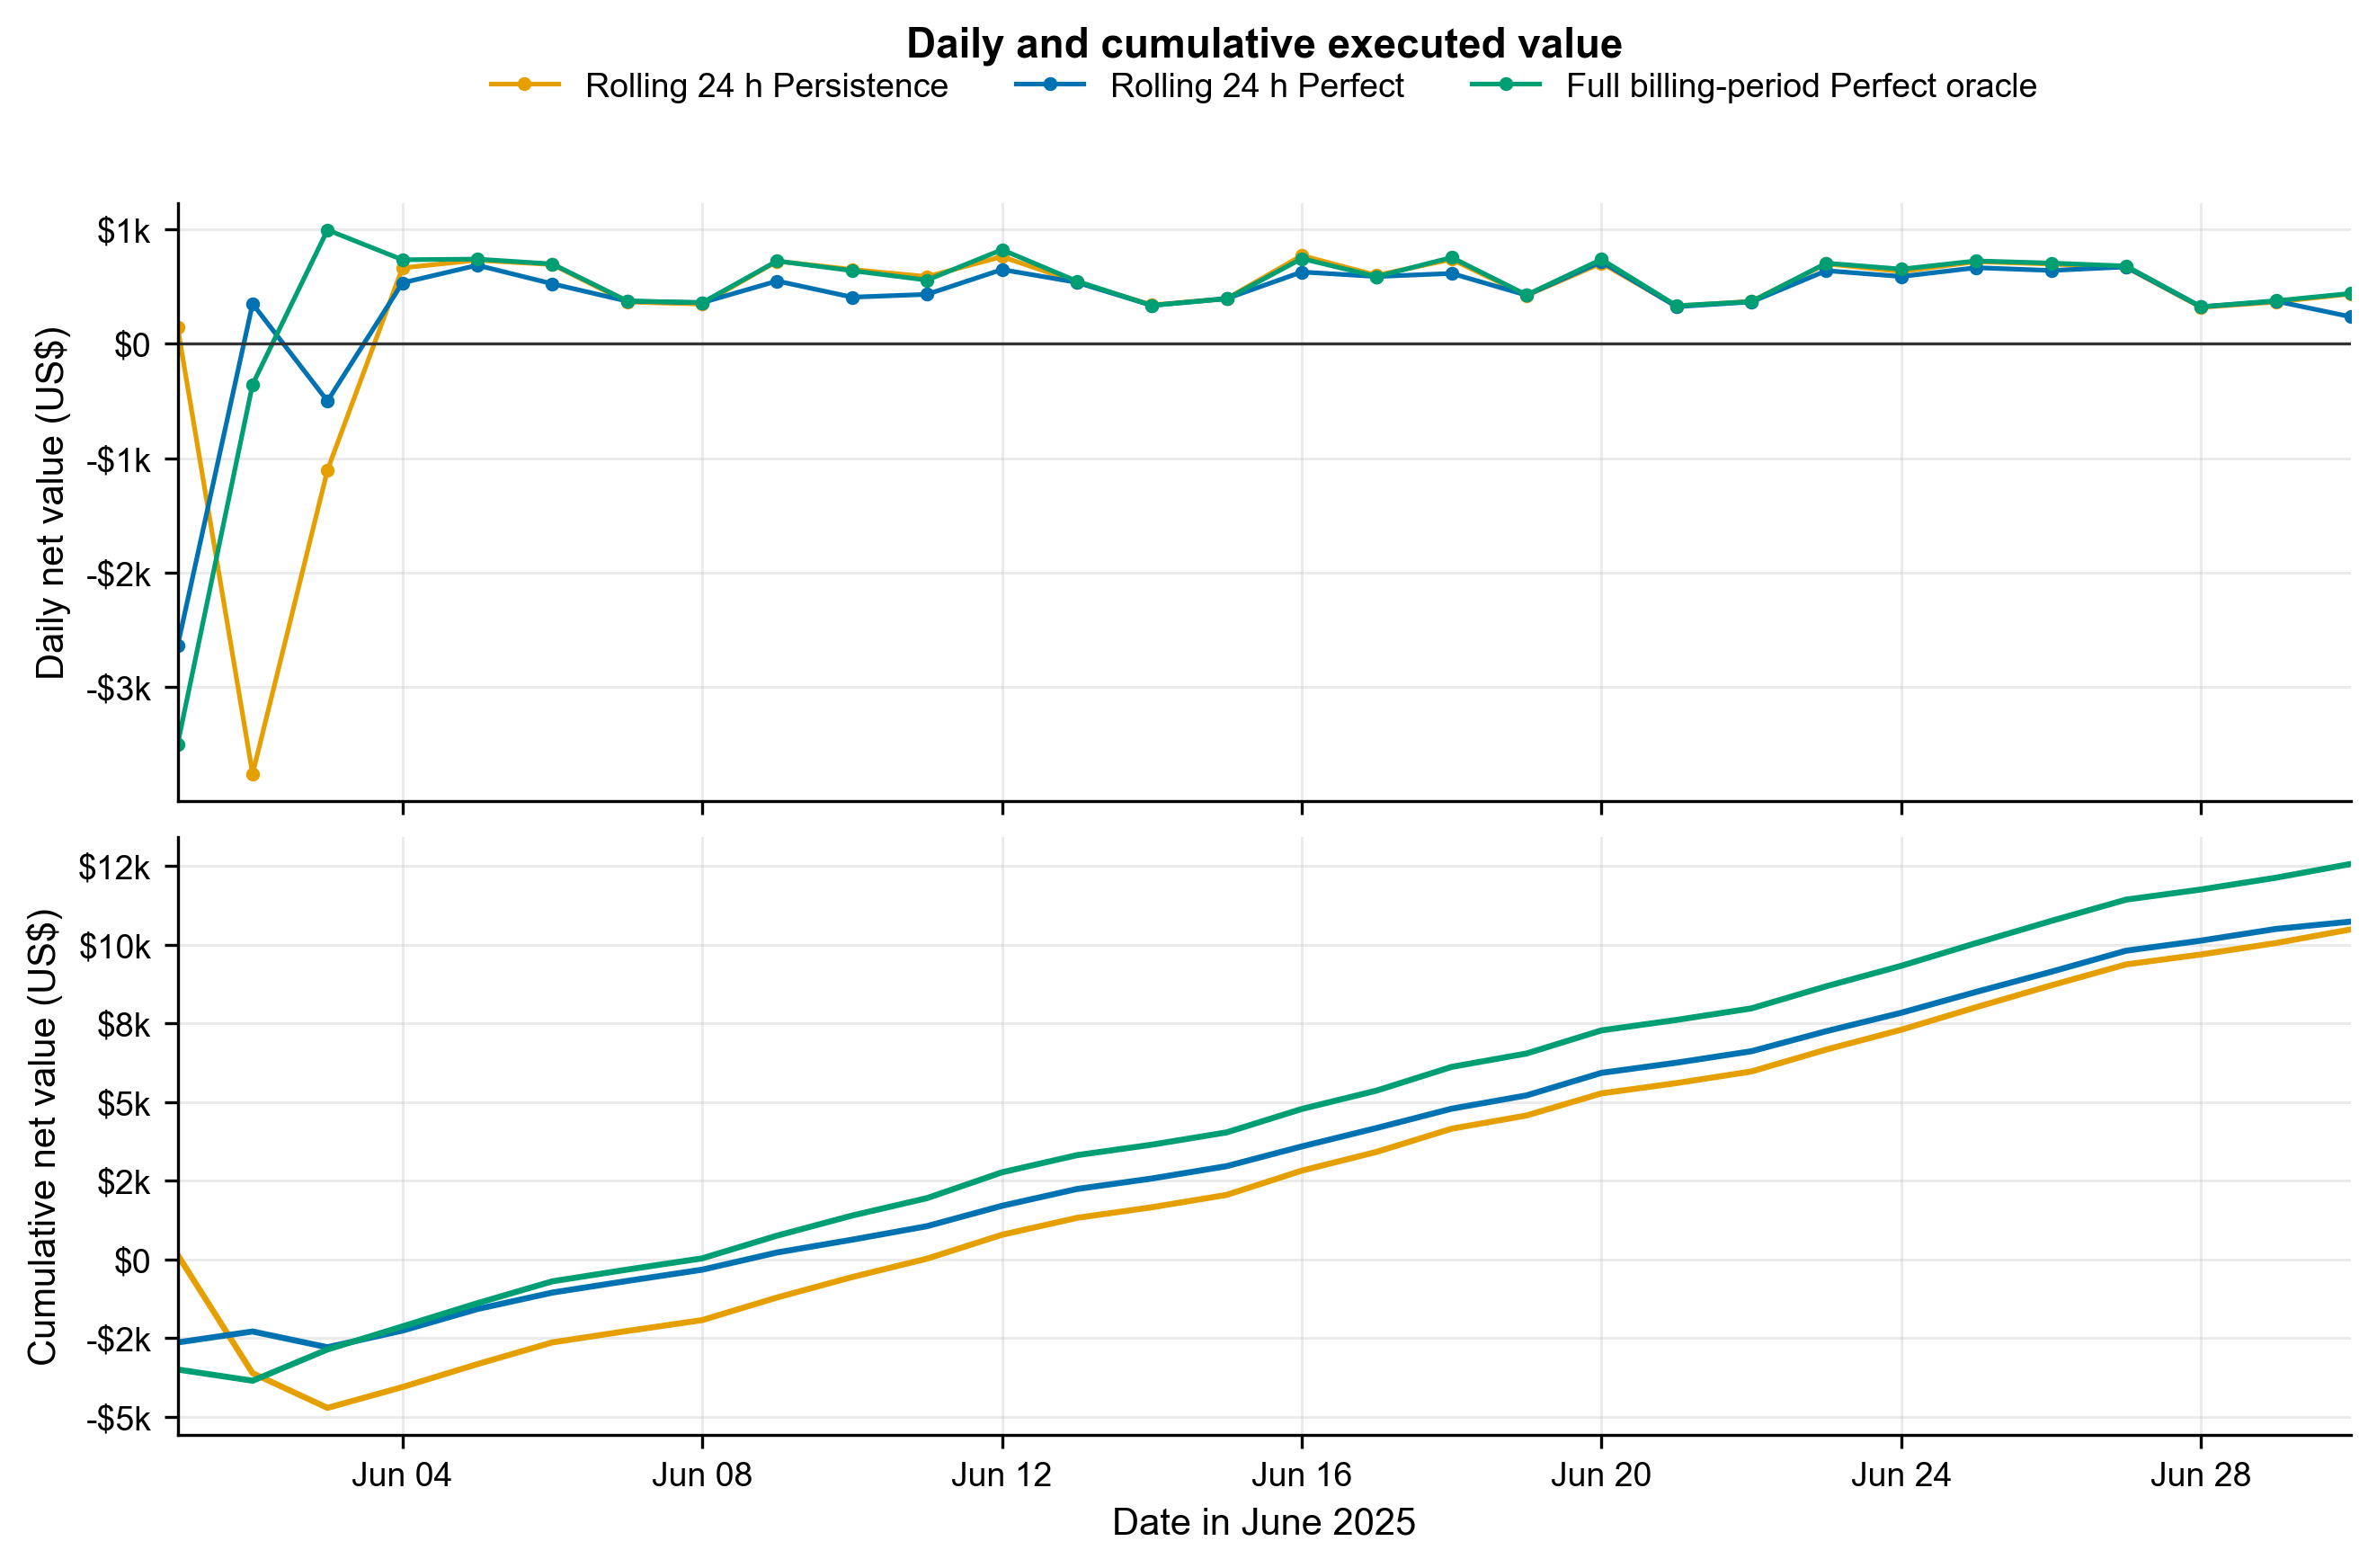
\includegraphics[width=0.96\textwidth]{fig_02_daily_rolling_oracle_value.png}
  \caption{Daily and cumulative executed net value for Rolling Persistence, Rolling Perfect, and the full-period Perfect oracle.}
  \label{fig:daily_financial}
\end{figure*}

\subsection{Resource and service-channel attribution}
The net-value decomposition in Fig.~\ref{fig:resource_decomposition} attributes
each 24-h policy's executed value to wholesale-market (WM) and non-wholesale
(NWM) channels, EV and BESS resources, and energy and capacity services. This
view reveals the mechanism hidden by a single wholesale-revenue total. WM
energy and capacity contributions are positive for all four policies, while
the NWM capacity attribution can be negative because market-oriented operation
changes the retail-meter trajectory and monthly demand-charge exposure.

\begin{figure*}[!t]
  \centering
  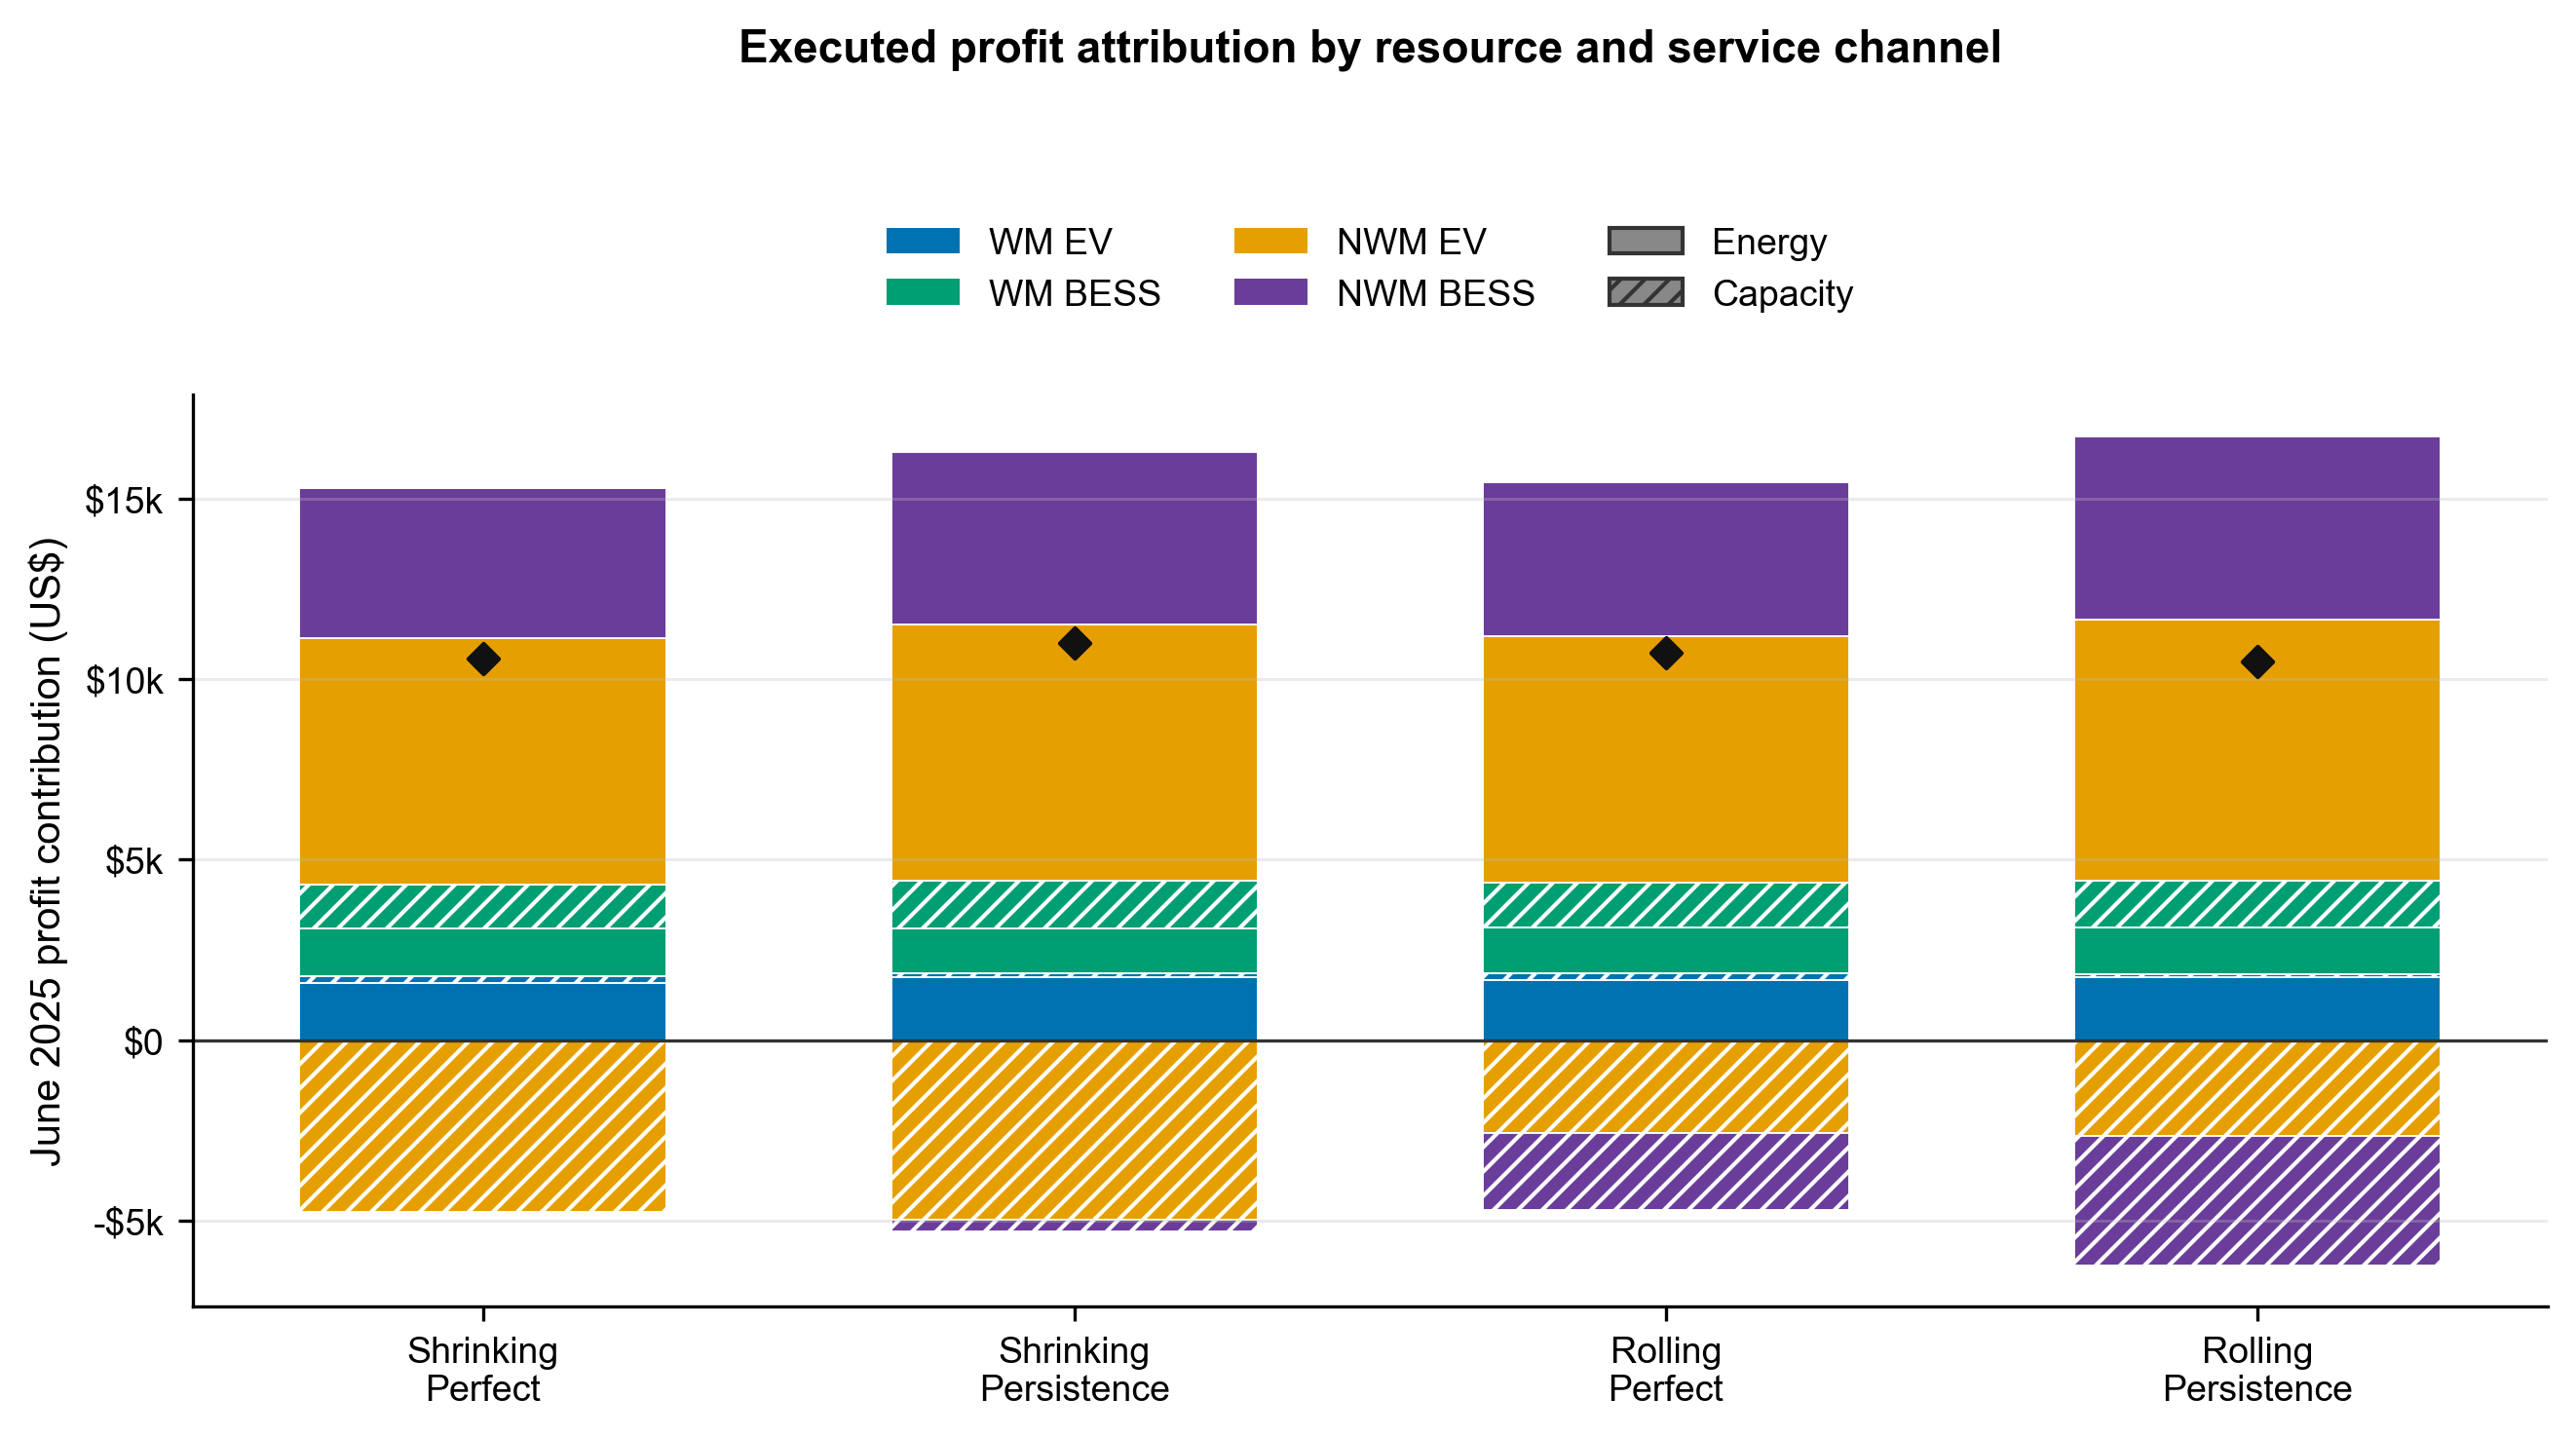
\includegraphics[width=0.96\textwidth]{fig_03_monthly_resource_service_decomposition.png}
  \caption{June 2025 executed-value attribution for the four 24-h policies. Color distinguishes WM/NWM and EV/BESS channels; hatching distinguishes energy and capacity components. Black diamonds show total net value.}
  \label{fig:resource_decomposition}
\end{figure*}

The daily decomposition is provided in Appendix~\ref{app:daily_decomposition}.
It shows that most operating days make positive contributions, whereas a small
number of days establish or increase the billing-period demand threshold and
therefore carry large negative NWM capacity terms.

\subsection{Numerical acceptance}
The numerical audit is retained as reproducibility evidence rather than as a
paper result figure. The largest formal meter residual is approximately
$10^{-8}$ kW, the largest settlement-identity residual approximately
$10^{-7}$ kW, and actual up/down-capability violations are of order
$10^{-11}$ kW. All are below the $10^{-6}$ kW acceptance tolerance. Every
Rolling solve terminates with Gurobi status 2 and CVXPY status
\texttt{optimal}; the maximum recorded relative gap is 0.999899\%. Detailed
daily residual, solver-gap, and stress-day plots are archived with the
versioned validation outputs and are not presented as economic result figures.

\section{Discussion}
\label{sec:discussion}

\subsection{What is validated}
The evidence supports correctness of the \emph{reported implementation} within
the stated tolerances: complete interval coverage; accepted solver status;
meter, settlement, and capability identities; nonnegative actual AS; equal EV
service; final SOC; and financial reconstruction. The full-period benchmark
also confirms that the 24-h policies leave economically relevant value outside
their look-ahead.

This does not prove that every modeling assumption is a market rule. Expected
AS deployment factors, the common 0.5-h duration guard, the retail export
credit, EV baseline construction, and known price trajectories remain explicit
assumptions. The distinction is important for a rigorous journal claim:
numerical implementation correctness and external market fidelity are related
but separate questions.

\subsection{Implications for forecast and sensitivity studies}
The oracle gap identifies horizon value, not solely forecast value. Therefore,
future forecast sensitivity should use matched initial SOC, monthly thresholds,
and DA commitments when the purpose is to isolate RT forecast effects. For
deployment studies, the more relevant metric is the closed-loop billing-period
value of each policy, where state paths are allowed to diverge.

The next sensitivity analysis activates passive building load and PV through
\eqref{eq:meter}. Because these resources alter the signed meter but not the
decision set, the base EV--BESS case remains intact and directly comparable.
The main robustness questions are whether (i) oracle advantage, (ii) retail cost
offsets to WM revenue, and (iii) daily feasibility conclusions persist across
PV/load scale and forecast cases.

\subsection{Generalizable findings}
Three findings define the paper's contribution. First, the retail meter materially
changes the value of a market-facing schedule, so gross WM revenue is not a
reliable controller metric. Second, the full-period oracle improves value
primarily by coordinating retail and wholesale states across the billing
period, not by maximizing a single revenue account. Third, ``Perfect forecast''
is not synonymous with ``upper bound'' under truncated economic MPC; the upper
bound requires the full feasible horizon and common boundary conditions.

\section{Limitations and future work}
\label{sec:limitations}

The study uses one month of workplace EV data, and essentially no overnight EV
carryover is represented. Prices are treated as known exogenous trajectories.
EVs are aggregated rather than mapped to station-specific electrical limits.
BESS degradation is represented only indirectly through efficiency and
throughput constraints. The wholesale model uses expected AS deployment and
does not reproduce regulation mileage, performance scores, no-pay charges,
telemetry, minimum bid sizes, scheduling-coordinator requirements, or every
CAISO settlement rule. The full-period benchmark is solved to a 1\% MIP gap,
not proven to exact global optimality.

Future work should: (i) repeat the validated base case across additional
seasons; (ii) add the passive PV/building sensitivity without replacing the
base case; (iii) introduce product-specific AS duration and activation models;
(iv) examine alternative EV baselines; (v) test forecast models beyond
Persistence using matched-state experiments and closed-loop billing-period
evaluation; and (vi) model station/network topology when site-level data become
available.

\section{Conclusion}
\label{sec:conclusion}

An EV--BESS portfolio behind a campus meter must be evaluated as one coupled
physical and financial system. The proposed framework preserves mandatory EV
service, BESS feasibility, signed retail-meter accounting, fixed DA
commitments, signed RT adjustments, actual nonnegative AS, and executed
first-step revenue reconstruction. In the validated June 2025 case, the
full-period Perfect benchmark produces \$12,565.15, 14.38\% more than the best
24-h policy. All formal solver, physical, financial, and graphical checks pass.
The result establishes a defensible benchmark and a reproducible validation
standard for the next PV/building and forecast-robustness analyses.

\section*{Acknowledgements and AI-assisted preparation disclosure}
The authors acknowledge the UCSD and TotalEnergies collaboration supporting the
campus EV--BESS modeling and validation workflow. AI-assisted tools were used
for language revision, document organization, and code-supported figure
generation. The authors reviewed the model statements, numerical provenance,
citations, and final manuscript and remain responsible for the content.

\appendix

\section{Complete financial objective and accounting identity}
\label{app:objective}

For a full evaluation set $\calT$, the oracle objective corresponding to
\eqref{eq:objective} is
\begin{align}
\min_{\boldsymbol{x}\in\mathcal{X}(\omega)}
J_{\calT}
={}&\sum_{t\in\calT} C_t^{\TOU}p_t^{\GI}\dt
+C^{\PD}z^{\PD}+C^{\NCD}z^{\NCD}\nonumber\\
&-\sum_{t\in\calT}C^{\EV}p_t^{\EV}\dt\nonumber\\
&-\sum_{t\in\calT}\dt
\left(\lambda_t^{\DA}p_t^{\DA}
+\lambda_t^{\RT}p_t^{\RT}\right)\nonumber\\
&-\sum_{t\in\calT}\sum_{x\in\calK}
\dt\,\rho_t^{x,\DA}c_t^{x,\DA}\nonumber\\
&-\sum_{t\in\calT}\sum_{x\in\calK}
\dt\,\rho_t^{x,\RT}c_t^{x,\RT}
-R^{\mathrm{deploy}}. \label{eq:full_objective}
\end{align}
The financial post-processor stores costs with negative signs. After independent
cent rounding by day, the validation accepts
\begin{align}
\left|V-(R^{\EV}+R^{\WM}+C^{\TOU}+C^{\PD}+C^{\NCD})\right|
\le \$0.03. \label{eq:rounding}
\end{align}

\section{Daily resource and service-channel attribution}
\label{app:daily_decomposition}

\begin{figure*}[!t]
  \centering
  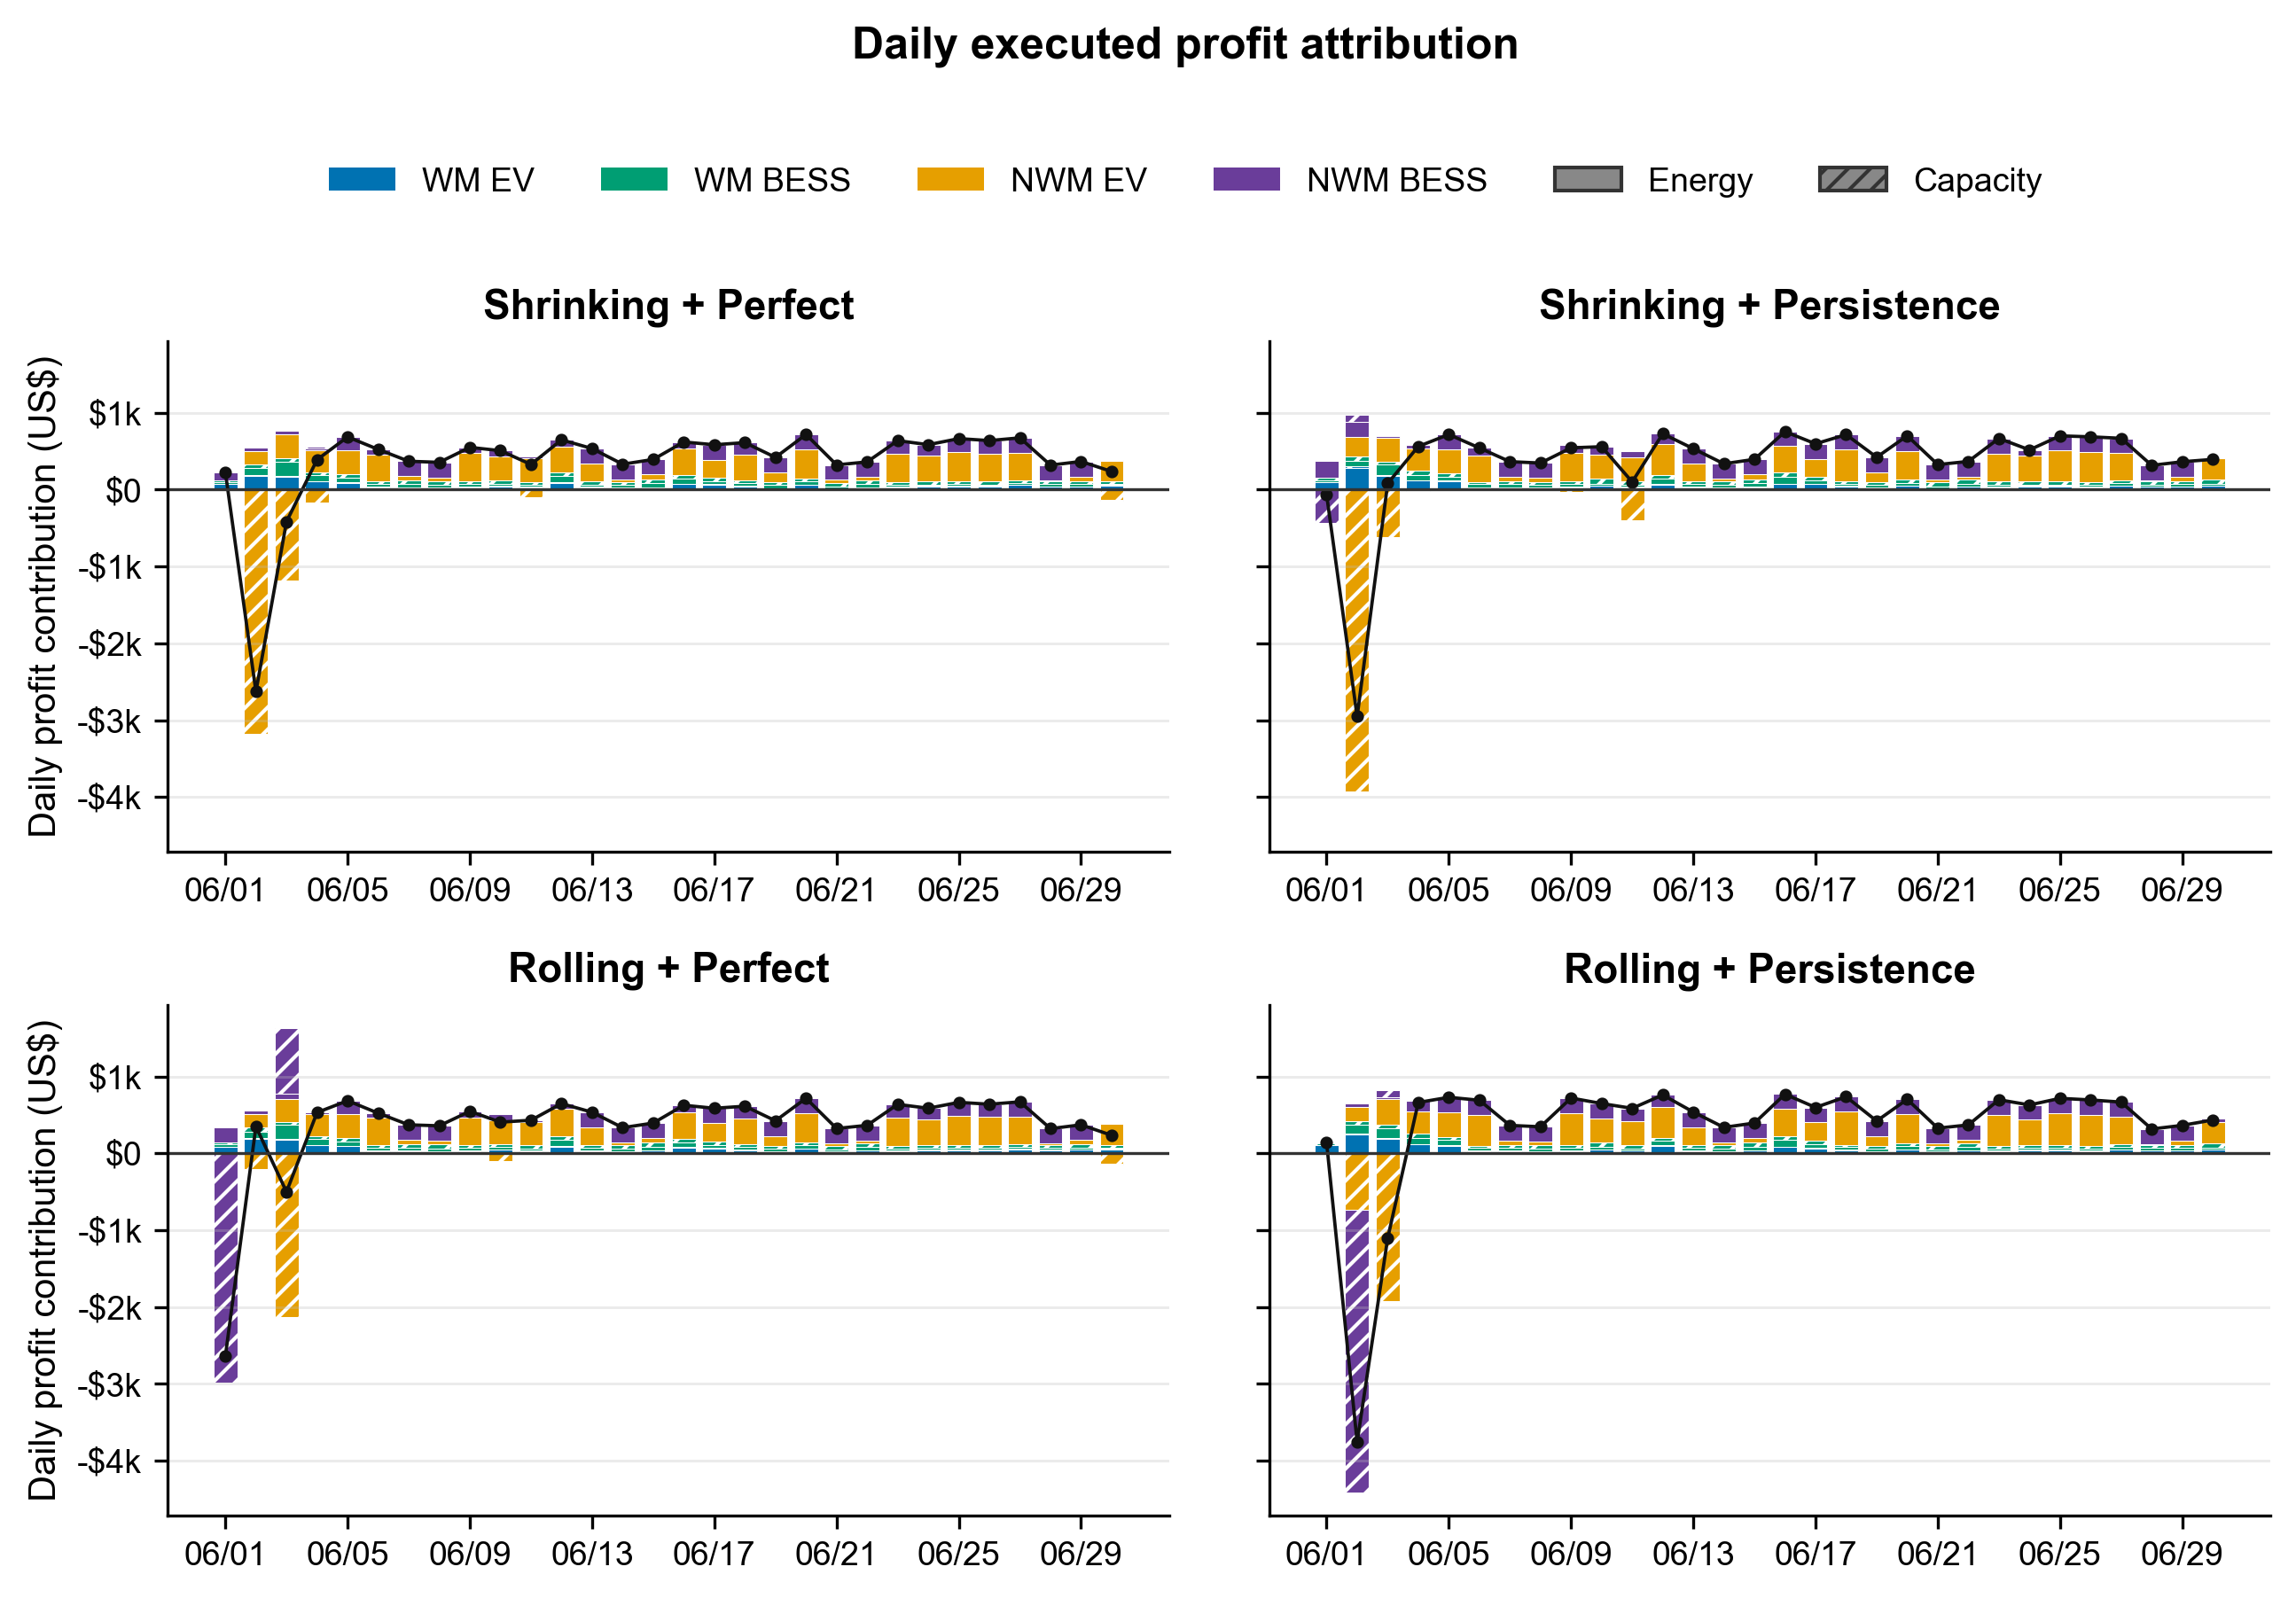
\includegraphics[width=\textwidth]{fig_04_daily_resource_service_decomposition.png}
  \caption{Daily executed-value attribution for the four 24-h policies. The black trace is daily net value; stacked bars separate WM/NWM, EV/BESS, and energy/capacity contributions.}
  \label{fig:daily_decomposition}
\end{figure*}

\clearpage
\bibliographystyle{elsarticle-num}
\bibliography{references_v2.7}

\end{document}
